\documentclass[11pt,class=report,crop=false]{standalone}
\usepackage[screen]{../python}

\begin{document}

%====================================================================
\chapitre{Main functions}
%====================================================================


%%%%%%%%%%%%%%%%%%%%%%%%%%%%%%%%%%%%%%%%%%%%%%%%%%%%
\section{Mathematics}

\textbf{Classical operations}
\begin{itemize}
  \item \ci{a + b},\quad\ci{a - b},\quad\ci{a * b}\quad classic operations
  \item \ci{a / b}\quad \og{}real\fg{} division (returns a floating point number)
  \item \ci{a // b}\quad Euclidean division quotient (returns an integer)
  \item \ci{a \% b}\quad remainder of the Euclidean division, called $a$ modulo $b$
  \item \ci{abs(x)}\quad absolute value
  \item \ci{x ** n}\quad power $x^n$
  \item \ci{4.56e12}\quad for $4.56 \times 10^{12}$
\end{itemize}

\bigskip

\textbf{\og{}math\fg{} module}

The use of other mathematical functions requires the \ci{math} module which is called by the command:
\mycenterline{\ci{from math import *}}

\begin{itemize}
  \item \ci{sqrt(x)}\quad square root $\sqrt{x}$
  \item \ci{cos(x)},\quad\ci{sin(x)},\quad\ci{tan(x)}\quad trigonometric functions $\cos x$, $\sin x$, $\tan x$ in radians
  \item \ci{pi}\quad approximate value of $\pi = 3.14159265\ldots$
  \item \ci{floor(x)}\quad integer just below $x$
  \item \ci{ceil(x)}\quad integer just above $x$
  \item \ci{gcd(a,b)}\quad gcd of $a$ and $b$
 \end{itemize}
 \bigskip

\textbf{\og{}random\fg{} module}

The \ci{random} module generates numbers in a pseudo-random way. It is called by the command:
\mycenterline{\ci{from random import *}}

\begin{itemize}
  \item \ci{random()}\quad on each call, returns a floating number $x$ at random, satisfying $0 \le x < 1$.
  \item \ci{randint(a,b)} \quad for each call, returns an integer $n$ at random, satisfying $a \le n \le b$.
  \item \ci{choice(mylist)} \quad on each call, randomly draws an item from the list.
  \item \ci{mylist.shuffle()} \quad mixes the list (the list is modified).
 \end{itemize}

\bigskip

\textbf{Binary notation}

\begin{itemize}
  \item \ci{bin(n)}\quad returns the binary notation of the integer $n$ as a string. 
  Example: \ci{bin(17)} returns \ci{'0b10001'}.
  
  \item To write a number directly in binary notation, simply write the number starting with \ci{0b} (without quotation marks). For example \ci{0b11011} is equal to \ci{27}.
 \end{itemize}




%%%%%%%%%%%%%%%%%%%%%%%%%%%%%%%%%%%%%%%%%%%%%%%%%%%%
\section{Booleans}

A boolean is a data that takes either the value \ci{True} or the value \ci{False}.

  
\bigskip

\textbf{Comparisons}
 
The following comparison tests return a boolean.
  \begin{itemize}
    \item \ci{a == b} \quad equality test
    	\item \ci{a < b} \quad strict lower test
    	\item \ci{a <= b} \quad large lower test
    	\item \ci{a > b} \quad or \quad \ci{a >= b}\quad higher test
    	\item \ci{a \!= b} \quad non-equality test
  \end{itemize}
  
 Do not confuse \og{}\ci{a = b}\fg{} (assignment) and \og{}\ci{a == b}\fg{} (equality test).
  
\bigskip
  
\textbf{Boolean operations}
  \begin{itemize}
    \item \ci{P and Q} \quad \quad logical \og{}and\fg{}
    	\item \ci{P or Q} \quad logical \og{}or\fg{}
    	\item \ci{not P} \quad negation
  \end{itemize} 
  
  
%%%%%%%%%%%%%%%%%%%%%%%%%%%%%%%%%%%%%%%%%%%%%%%%%%%%
\section{Strings I}

\textbf{Strings}

\begin{itemize}
  \item \ci{"A"} \quad or \quad \ci{'A'} \quad one character
  \item \ci{"Python"}\quad or \quad \ci{'Python'} \quad a string
  \item \ci{len(string)}\quad the string length. Example: \ci{len("Python")} returns $6$.
  \item \ci{string1 + string2}\quad concatenation.   
  
  Example: \ci{"I love" + "Python"} returns \ci{"I lovePython"}.
  
  \item \ci{string[i]}\quad returns the $i$-th character of \ci{string} (numbering starts at $0$). 
  
  Example with \ci{string = "Python"}, \ci{string[1]} is equal to \ci{"y"}. See the table below.
\end{itemize}

\begin{center}
\begin{tabular}{|c||c|c|c|c|c|c|}
\hline
Letter & \textbf{P} & \textbf{y} & \textbf{t} & \textbf{h} & \textbf{o} & \textbf{n} \\ \hline
Rank & 0 & 1 & 2 & 3 & 4 & 5 \\ \hline
\end{tabular}
\end{center}


\textbf{Number/string conversion}

\begin{itemize}
  \item \textbf{String.} \ci{str(number)}\quad converts a number (integer or floating point number) into a string.
  Examples: \ci{str(7)} returns the string \ci{"7"}; \ci{str(1.234)} returns the string \ci{"1.234"}.
  
  \item \textbf{Integer.} \ci{int(string)}\quad returns the integer corresponding to the string. Example: \ci{int("45")} returns the integer \ci{45}.
  
   \item \textbf{Floating point number.} \ci{float(string)}\quad returns the floating point number corresponding to the string. Example: \ci{float("3.14")} returns the number \ci{3.14}. 
 \end{itemize}  


\bigskip

\textbf{Substrings}

\begin{itemize}
  \item \ci{string[i:j]}\quad returns the substring of characters with from rank $i$ to rank $j-1$ of \ci{string}.
  
   Example: with \ci{string = "This is a string"}, \ci{string[2:7]} returns \ci{"is is"}.
   
  \item \ci{string[i:]}\quad returns characters from rank $i$ until the end of \ci{string}. 
  
  Example:
  \ci{string[5:]} returns \ci{"is a string"}.
  
  \item\ci{string[:j]}\quad returns characters from the beginning to rank $j-1$ of \ci{string}. Example: \ci{string[:4]} returns \ci{"This"}.
  
\end{itemize}


\bigskip
\textbf{Format}

The \ci{format()} method allows you to format text or numbers. This function returns a string.

\begin{itemize}
  \item \textbf{Text}
  
  \begin{center}
 \lstinline[showspaces=true]!Test      ! \qquad\qquad
    \lstinline[showspaces=true]!      Test!  \qquad\qquad
 \lstinline[showspaces=true]!   Test   !   
 \end{center}
 
  \begin{itemize}
    \item \ci{'\{:10\}'.format('Test')} \quad left alignment (on 10 characters)
    \item \ci{'\{:>10\}'.format('Test')} \quad right alignment
    \item \ci{'\{:\^10\}'.format('Test')} \quad centered 
  \end{itemize}

  \item \textbf{Integer}
  
  \begin{center}
 \lstinline[showspaces=true]!456! \qquad\qquad
    \lstinline[showspaces=true]!   456!  \qquad\qquad
 \lstinline[showspaces=true]!000456!   
 \end{center}
 
  \begin{itemize}
    \item \ci{'\{:d\}'.format(456)} \quad integer  
    \item \ci{'\{:6d\}'.format(456)} \quad right aligned (on 6 characters)
    \item \ci{'\{:06d\}'.format(456)} \quad adding leading zeros (on 6 characters)
  \end{itemize} 
  
  \item \textbf{Floating point number}
  
  \begin{center}
 \lstinline[showspaces=true]!3.141593! \qquad\qquad
    \lstinline[showspaces=true]!3.14159265!  \qquad\qquad
 \lstinline[showspaces=true]!  3.1416!  \qquad\qquad
 \lstinline[showspaces=true]!003.1416!   
 \end{center}
 
  \begin{itemize}
    \item \ci{'\{:f\}'.format(3.14159265653589793)} \quad floating point number 
    \item \ci{'\{:.8f\}'.format(3.14159265653589793)} \quad $8$ decimal places 
    \item \ci{'\{:8.4f\}'.format(3.14159265653589793)} \quad on $8$ characters with $4$ numbers after the decimal point 
    \item 
    \ci{'\{:08.4f\}'.format(3.141592653589793)} \quad adding leading zeros 
  \end{itemize}   
   
\end{itemize}



%%%%%%%%%%%%%%%%%%%%%%%%%%%%%%%%%%%%%%%%%%%%%%%%%%%%
\section{Strings II}



\textbf{Encoding}

\begin{itemize}
  \item \ci{chr(n)} \quad returns the character associated with the ASCII/unicode code number $n$. Example: \ci{chr(65)} returns \ci{"A"}; \ci{chr(97)} returns \ci{"a"}.
    
  \item \ci{ord(c)} \quad returns the ASCII/unicode code number associated with the character $c$. Example: \ci{ord("A")} returns \ci{65}; \ci{ord("a")} returns \ci{97}.
\end{itemize}

The beginning of the ASCII/unicode table is given below.

\myfigure{0.8}{
\small
  \tikzinput{../strings/strings-unicode}
} 

\bigskip

\textbf{Upper/lower-case}

\begin{itemize}
  \item \ci{string.upper()} returns a string in uppercase.
  \item \ci{string.lower()} returns a string in lowercase.  
\end{itemize}

\bigskip

\textbf{Search/replace}

\begin{itemize}
  \item \ci{substring in string} \quad returns \og{}true\fg{} or \og{}false\fg{} depending on if \ci{substring} appears in \ci{string}.
  
   Example:
\ci{"NOT" in "TO BE OR NOT TO BE"} returns \ci{True}.

  \item \ci{string.find(substring)} \quad returns the rank at which the substring was found (and \ci{-1} otherwise).
  
  Example: with \ci{string = "ABCDE"}, \ci{string.find("CD")} returns \ci{2}.
  
   \item \ci{string.replace(substring,new_substring)} \quad replaces 
   each occurrence of the substring by the new substring.
   
   Example: with \ci{string = "ABCDE"}, \ci{string.replace("CD","XY")} returns
   \ci{"ABXYE"}.

\end{itemize}


\bigskip

\textbf{Split/join}

\begin{itemize}
  \item \ci{string.split(separator)} \quad separates the string into a list of substrings (by default the separator is the space).
  
  Examples: 
  \begin{itemize}  
 
    \item \ci{"To be or not to be.".split()} returns \ci{['To', 'be', 'or', 'not', 'to', 'be.']}
        \item \ci{"12.5;17.5;18".split(";")} returns \ci{['12.5', '17.5', '18']}
  \end{itemize}   
  
   \item \ci{separator.join(mylist)} \quad groups the substrings into a single string by adding the separator between each.

   Examples:
   
     \begin{itemize}  
       \item \ci{"".join(["To", "be", "or", "not", "to", "be."])} returns the string \ci{'Tobeornottobe.'} Spaces are missing.
       \item \ci{" ".join(["To", "be", "or", "not", "to", "be."])} returns \ci{'To be or not to be.'} It's better when the separator is a space.
       \item \ci{"--".join(["To", "be", "or", "not", "to", "be."])} returns the string  \ci{'To--be--or--not--to--be.'}  
     \end{itemize}
 

\end{itemize}


%%%%%%%%%%%%%%%%%%%%%%%%%%%%%%%%%%%%%%%%%%%%%%%%%%%%
\section{Lists I}

\textbf{Construction of a list}

Examples:
\begin{itemize}
    \item \ci{mylist1 = [5,4,3,2,1]} \quad a list of five integers.
    \item \ci{mylist2 = ["Friday","Saturday","Sunday"]} \quad a list of three strings.
    \item \ci{mylist3 = []} \quad the empty list.
    \item \ci{list(range(n))} \quad list of integers from $0$ to $n-1$.
    \item \ci{list(range(a,b))} \quad list of integers from $a$ to $b-1$.
    \item \ci{list(range(a,b,step))} \quad list of integers from $a$ to $b-1$, with a step given by the integer \ci{step}.
  \end{itemize}
  
\bigskip
 
\textbf{Get an item}

\begin{itemize}
    \item \ci{mylist[i]} \quad returns the element at rank $i$. Be careful, the rank starts at $0$.

Example: \ci{mylist = ["A","B","C","D","E","F"]} then \ci{mylist[2]} returns \ci{"C"}.

\medskip
 \begin{center}
\begin{tabular}{|c||c|c|c|c|c|c|}
\hline
Letter & \textbf{"A"} & \textbf{"B"} & \textbf{"C"} & \textbf{"D"} & \textbf{"E"} & \textbf{"F"} \\ \hline
Rank & 0 & 1 &2 & 3 & 4 & 5 \\ \hline
\end{tabular}
\end{center}
\medskip

    \item \ci{mylist[-1]} \quad returns the last element, \ci{mylist[-2]} returns the second last element\ldots
    
    
    \item \ci{mylist.pop()} \quad removes the last item from the list and returns it.
\end{itemize}


\bigskip

\textbf{Add one element (or more)} 

\begin{itemize}

    \item \ci{mylist.append(element)} \quad adds the item at the end of the list.
    Example: if \ci{mylist = [5,6,7,8]} then 
  \ci{mylist.append(9)} adds $9$ to the list, \ci{mylist} is now \ci{[5,6,7,8,9]}.
  
    \item \ci{new_mylist = mylist + [element]} \quad provides a new list with an extra element at the end. Example: \ci{[1,2,3,4] + [5]} is \ci{[1,2,3,4,5]}.
    \item \ci{[element] + mylist} \quad returns a list where the item is added at the beginning. Example: \ci{[5] + [1,2,3,4]} is \ci{[5,1,2,3,4]}. 
     \item \ci{mylist1 + mylist2} \quad concatenates the two lists. 
     Example: with \ci{mylist1 = [4,5,6]} and \ci{mylist2 = [7,8,9]} then \ci{mylist1 + mylist2} is \ci{[4,5,6,7,8,9]}.
\end{itemize}

\bigskip

\textbf{Example of construction.} Here is how to build the list that contains the first squares:
   \begin{center}
  \begin{minipage}{0.9\textwidth}
\begin{lstlisting}
list_squares = []               # We start from an empty list
for i in range(10):
    list_squares.append(i**2)     # We add squares one by one
\end{lstlisting}
  \end{minipage}
  \end{center}  
At the end \ci{list_squares} is:
\mycenterline{\ci{[0, 1, 4, 9, 16, 25, 36, 49, 64, 81]}}  


\bigskip
\textbf{Browse a list} 

\begin{itemize}
  \item \ci{len(mylist)} \quad returns the length of the list. Example: \ci{len([5,4,3,2,1])} returns $5$.
    
  \item Browse a list (and here display each item):
\begin{lstlisting}
for element in mylist:
    print(element)
\end{lstlisting}

  \item Browse a list using the rank.
\begin{lstlisting}
n = len(mylist)
for i in range(n):
    print(i,mylist[i])
\end{lstlisting}  
\end{itemize}


%%%%%%%%%%%%%%%%%%%%%%%%%%%%%%%%%%%%%%%%%%%%%%%%%%%%
\section{Lists II}



\textbf{Mathematics}

   \begin{itemize}
    \item \ci{max(mylist)} \quad returns the largest element. Example: \ci{max([10,16,13,14])} returns \ci{16}.
    
    \item \ci{min(mylist)} \quad returns the smallest element. Example: \ci{min([10,16,13,14])} returns \ci{10}.
    
    \item \ci{sum(mylist)} \quad returns the sum of all elements. Example: \ci{sum([10,16,13,14])} returns \ci{53}.
\end{itemize}

\bigskip
    
\textbf{Slicing lists}
  
  \begin{itemize}
    \item \ci{mylist[a:b]} \quad returns the sublist of elements from rank $a$ to rank $b-1$.
    
    \item \ci{mylist[a:]} \quad returns the list of elements from rank $a$ until the end.
      
    \item \ci{mylist[:b]} \quad returns the list of items from the beginning to rank $b-1$.
    

\end{itemize}


\medskip
 \begin{center}
\begin{tabular}{|c|||c|c|c|c|c|c|c|}
\hline
Letter & \textbf{"A"} & \textbf{"B"} & \textbf{"C"} & \textbf{"D"} & \textbf{"E"} & \textbf{"F"} & \textbf{"G"} \\ \hline
Rank & 0 & 1 & 2 & 3 & 4 & 5 & 6 \\ \hline
\end{tabular}
\end{center}
\medskip
  
    For example if \ci{mylist = ["A","B","C","D","E","F","G"]} then:
  \begin{itemize}
    \item \ci{mylist[1:4]} \quad returns \ci{["B","C","D"]}.
    \item \ci{mylist[:2]} \quad is like \ci{mylist[0:2]} and returns \ci{["A","B"]}.   
    \item \ci{mylist[4:]} \quad returns \ci{["E","F","G"]}.  It's the same thing 
     as \ci{mylist[4:n]} where \ci{n = len(mylist)}.
  \end{itemize} 

\bigskip

\textbf{Find the rank of an element} 

\begin{itemize}

    \item   
   \ci{mylist.index(element)} returns the first position at which the item was found. Example: with \ci{mylist = [12, 30, 5, 9, 5, 21]},
   \ci{mylist.index(5)} returns $2$.

  \item If you just want to know if an item belongs to a list, then the statement:  
  \mycenterline{\ci{element in mylist}}  
  
  returns \ci{True} or \ci{False}.
  Example: with \ci{mylist = [12, 30, 5, 9, 5, 21]},
   \og\ci{9 in mylist}\fg{} is true, while \og\ci{8 in mylist}\fg{} is false.
  
\end{itemize}

\bigskip

\textbf{Order}

\begin{itemize}
  \item \ci{sorted(mylist)} \quad returns the ordered list of items.
  
   Example: \ci{sorted([13,11,7,4,6,8,12,6])} returns the list \ci{[4,6,6,7,8,11,12,13]}.
   
   \item \ci{mylist.sort()} \quad does not return anything but the list \ci{mylist} is now ordered.
\end{itemize}


\bigskip

\textbf{Invert a list}

Here are three methods:
\begin{itemize}
  \item \ci{mylist.reverse()} \quad modifies the list in place;
  \item \ci{list(reversed(mylist))} \quad returns a new list;
  \item \ci{mylist[::-1]} \quad returns a new list. 
\end{itemize}  


\bigskip

\textbf{Delete an item}

Three methods.
\begin{itemize}
  \item \ci{mylist.remove(element)} \quad deletes the first occurrence found.
  
   Example: \ci{mylist = [2,5,3,8,5]}, the instruction \ci{mylist.remove(5)} modifies the list which is now \ci{[2,3,8,5]} (the first $5$ has disappeared).
  
   \item \ci{del mylist[i]} \quad deletes element at rank $i$ (the list is modified).
   
   \item \ci{element = mylist.pop()} \quad removes the last item from the list and returns it.
\end{itemize}


\bigskip

\textbf{List comprehension}

  \begin{itemize}
    \item Let's start from a list, for example \ci{mylist = [1,2,3,4,5,6,7,6,5,4,3,2,1]}.
    
    \item \ci{list_doubles = [ 2*x for x in mylist ]} \quad returns a list that contains the doubles of the items of \ci{mylist}. So this is the list \ci{[2,4,6,8,...]}.
    
    \item \ci{liste_squares = [ x**2 for x in mylist ]} \quad returns the list of squares of the items in the list \ci{mylist}. So this is the list \ci{[1,4,9,16,...]}.
    
    \item \ci{partial_list = [ x for x in mylist if x > 2 ]} \quad
    extracts from the list only the elements greater than $2$. So this is the list \ci{[3,4,5,6,7,6,5,4,3]}.
	\end{itemize}
	
\bigskip	 

\textbf{List of lists}
  
Example: 
  \mycenterline{\ci{array = [ [2,14,5], [3,5,7], [15,19,4], [8,6,5] ]}}
  corresponds to the table:
  \myfigure{0.7}{
  \tikzinput{fig-tableau}
}
  Then \ci{array[i]} returns the sublist of rank $i$, and
  \ci{array[i][j]} returns the element located in the sublist number $i$, at rank $j$  of this sublist. For example:
  \begin{itemize}
  \item \ci{array[0]} \quad returns the sublist \ci{[2,14,5]}.
  \item \ci{array[1]} \quad returns the sublist \ci{[3,5,7]}.
  \item \ci{array[0][0]} \quad returns the integer \ci{2}.
  \item \ci{array[0][1]} \quad returns the integer \ci{14}.
  \item \ci{array[2][1]} \quad returns the integer \ci{19}.
\end{itemize}

\medskip

A table of $n$ rows and $p$ columns.
\begin{itemize}
    \item \ci{array = [[0 for j in range(p)] for i in range(n)]} \quad initializes an array and fills it with $0$.
    \item \ci{array[i][j] = 1} \quad modifies a value in the table (the one at the location $(i,j)$).
\end{itemize}


%%%%%%%%%%%%%%%%%%%%%%%%%%%%%%%%%%%%%%%%%%%%%%%%%%%%
\section{Input/output}

\textbf{Display}

\begin{itemize}
  \item \ci{print(string1,string2,string3,...)} \quad displays strings or objects.
 Example: \ci{print("Value =",14)} displays \ci{Value = 14}.
 Example: \ci{print("Line 1 \\n Line 2")} displays on two lines.
 
  \item \textbf{Separator.} \ci{print(...,sep="...")} \quad changes the separator (by default the separator is the space character). Example: \ci{print("Bob",17,13,16,sep="; ")} displays
  \ci{Bob; 17; 13; 16}.
  
   \item \textbf{End of line.} \ci{print(...,end="...")} \quad changes the character placed at the end (by default it is the line break character \ci{\\n}).
   Example \ci{print(17,end="")} then \ci{print(76)} displays \ci{1776} on a single line.
   
\end{itemize}

\bigskip

\textbf{Keyboard entry}

\ci{input()} \quad pauses the program and waits for the user to send a message on the keyboard (ended by pressing the \og{}Enter\fg{} key). The message is a string.

Here is a small program that asks for the user's first name and age and displays a message like 
\og{}Hello Kevin\fg{} then \og{}You are a minor/adult\fg{} according to age. 
\begin{lstlisting}
first_name = input ("What's your name? ")
print("Hello",first_name)

age_str = input("How old are you? ")
age = int(age_str)

if age >= 18:
    print("You're an adult!")
else:
    print("You're a minor!")
\end{lstlisting}  




%%%%%%%%%%%%%%%%%%%%%%%%%%%%%%%%%%%%%%%%%%%%%%%%%%%%
\section{Files}

\textbf{Order} 

\begin{itemize}
  \item \ci{fi = open("my_file.txt","r")} \quad opening in reading (\ci{"r"} for read).
  \item \ci{fi = open("my_file.txt","w")} \quad opening in writing (\ci{"w"} for write). The file is created if it does not exist, if it existed the previous content is first deleted.
  \item \ci{fi = open("my_file.txt","a")} \quad opening for writing, the data will be written at the end of the current data (\ci{"a"} for append).
  
  \item \ci{fi.write("one line")} \quad write to the file.
  \item \ci{fi.read()} \quad reads the whole file (see below for another method).
  \item \ci{fi.readlines()} \quad reads all the lines (see below for another method).
  
  \item \ci{fi.close()} \quad file closing.
\end{itemize}

\bigskip

\textbf{Write lines to a file} 

\begin{lstlisting}
fi = open("my_file.txt","w")

fi.write("Hello world!\n")

line = "Hi there.\n"
fi.write(line)

fi.close()
\end{lstlisting}



\bigskip

\textbf{Read lines from a file} 

\begin{lstlisting}
fi = open("my_file.txt","r")

for line in fi:
    print(line)

fi.close()
\end{lstlisting}


\bigskip

\textbf{Read a file (official method)} 

\begin{lstlisting}
with open("my_file.txt","r") as fi: 
    for line in fi: 
        print(line) 
\end{lstlisting}


%%%%%%%%%%%%%%%%%%%%%%%%%%%%%%%%%%%%%%%%%%%%%%%%%%%%
\section{Turtle}

The \ci{turtle} module is called by the command:
\mycenterline{\ci{from turtle import *}}

\bigskip

\textbf{Main commands}

\begin{itemize}
  \item \ci{forward(length)} advances a number of steps
  \item \ci{backward(length)} goes backwards
  \item \ci{right(angle)} turns to the right (without advancing) at a given angle in degrees
  \item \ci{left(angle)} turns left
  \item \ci{setheading(direction)} points in a direction ($0$ = right, $90$ = top, $-90$ = bottom, $180$ = left)
  \item \ci{goto(x,y)} moves to the point $(x,y)$
  \item \ci{setx(newx)} changes the value of the abscissa
  \item \ci{sety(newy)} changes the value of the ordinate
  
  
  \item \ci{down()} sets the pen down
  \item \ci{up()} sets the pen up
  \item \ci{width(size)} changes the thickness of the line
  \item \ci{color(col)} changes the color: \ci{"red"}, \ci{"green"}, \ci{"blue"}, \ci{"orange"}, \ci{"purple"}\ldots
  
  \item \ci{position()} returns the $(x,y)$ position of the turtle
  \item \ci{heading()} returns the direction \ci{angle} to which the turtle is pointing
  \item \ci{towards(x,y)} returns the angle between the horizontal and the segment starting at the turtle and ending at the point $(x,y)$
  \item \ci{speed("fastest")} \quad maximum travel speed  
  \item \ci{exitonclick()} ends the program as soon as you click
\end{itemize}

\bigskip

\textbf{Several turtles}

Here is an example of a program with two turtles.
\begin{lstlisting}
turtle1 = Turtle()   # with capital 'T'!
turtle2 = Turtle()

turtle1.color('red')
turtle2.color('blue')

turtle1.forward(100)
turtle2.left(90)
turtle2.forward(100)
\end{lstlisting}



%%%%%%%%%%%%%%%%%%%%%%%%%%%%%%%%%%%%%%%%%%%%%%%%%%%%
\section{Matplotlib}

With the \ci{matplotlib} module it is very easy to draw a list. Here is an example.

\begin{center}
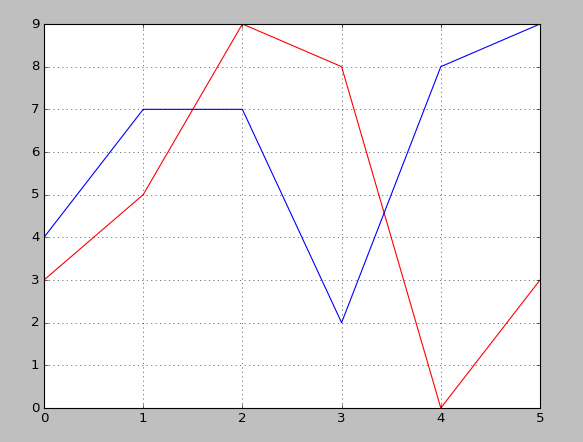
\includegraphics[scale=\myscale,scale=0.5]{../lists/screen-lists-lesson-visualization}
\end{center}

\begin{lstlisting}
import matplotlib.pyplot as plt

mylist1 = [3,5,9,8,0,3]
mylist2 = [4,7,7,2,8,9]

plt.plot(mylist1,color="red")
plt.plot(mylist2,color="blue")
plt.grid()
plt.show()
\end{lstlisting}


\textbf{Main functions.}

\begin{itemize}
  \item \ci{plt.plot(mylist)} traces the points of a list (in the form $(i,\ell_i)$)  that are joined by segments. 
  \item \ci{plt.plot(list_x,list_y)} traces the points of a list (of the form  $(x_i,y_i)$ where $x_i$ browses the first list and $y_i$ the second).    
  \item \ci{plt.scatter(x,y,color='red',s=100)} displays a point at $(x,y)$ (of a size \ci{s}).
  \item \ci{plt.grid()} draws a grid.  
  \item \ci{plt.show()} displays everything. 
  \item \ci{plt.close()} exits the display.
  
  \item \ci{plt.xlim(xmin,xmax)} defines the interval for the $x$.
  \item \ci{plt.ylim(ymin,ymax)} defines the interval for the $y$.
  \item \ci{plt.axis('equal')} imposes an orthonormal basis.  
\end{itemize}

%%%%%%%%%%%%%%%%%%%%%%%%%%%%%%%%%%%%%%%%%%%%%%%%%%%%
\section{Tkinter}

%---------------------------------------------------
\subsection{Graphics}

To display this:
\begin{center}
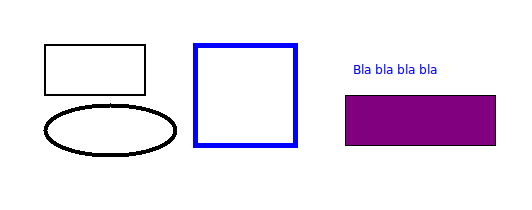
\includegraphics[scale=\myscale,scale=0.6]{../statistics/screen-stat-lesson-intro}
\end{center}
The code is:
\begin{lstlisting}
# tkinter window
root = Tk()
        
canvas = Canvas(root, width=800, height=600, background="white")
canvas.pack(fill="both", expand=True)

# A rectangle
canvas.create_rectangle(50,50,150,100,width=2)

# A rectangle with thick blue edges
canvas.create_rectangle(200,50,300,150,width=5,outline="blue")

# A rectangle filled with purple
canvas.create_rectangle(350,100,500,150,fill="purple")

# An ellipse
canvas.create_oval(50,110,180,160,width=4)

# Some text
canvas.create_text(400,75,text="Bla bla bla bla",fill="blue")

# Launch of the window
root.mainloop()
\end{lstlisting}


Some explanations:
\begin{itemize}
  \item The \ci{tkinter} module allows us to define variables \ci{root} and \ci{canvas} that determine a graphic window (here width $800$ and height $600$ pixels).
  Then describe everything you want to add to the window. And finally the window is displayed by the command \ci{root.mainloop()} (at the very end). 
  
    
  \item Attention! The window's graphic marker has its $y$-axis pointing downwards. The origin $(0,0)$ is the top left corner (see figure below). 
  
  \item Command to draw a rectangle: \ci{create_rectangle(x1,y1,x2,y2)}; just specify the coordinates $(x_1,y_1)$, $(x_2,y_2)$ of two opposite vertices. The option \ci{width} adjusts the thickness of the line, \ci{outline} defines the color of this line, \ci{fill} defines the filling color.
  
  \item An ellipse is traced by the command \ci{create_oval(x1,y1,x2,y2)}, where $(x_1,y_1)$, $(x_2,y_2)$ are the coordinates of two opposite vertices of a rectangle framing the desired ellipse (see figure). A circle is obtained when the corresponding rectangle is a square!  
  
  \item Text is displayed by the command \ci{canvas.create_text(x,y,text="My text")} specifying the coordinates $(x,y)$ of the point from which you want to display the text. 
  
\end{itemize}

\myfigure{0.8}{
\tikzinput{../statistics/fig-stat-lesson-intro}
}



%---------------------------------------------------
\subsection{Buttons}

It is more ergonomic to display windows where actions are performed by clicking on buttons.
Here is the window of a small program with two buttons. The first button changes the color of the rectangle, the second button ends the program.
\begin{center}
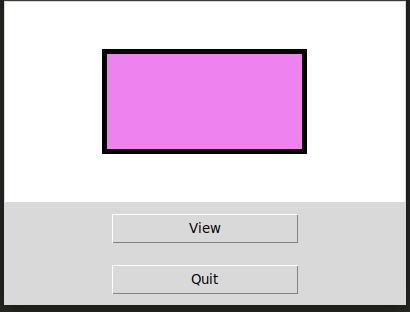
\includegraphics[scale=\myscale,scale=0.6]{../statistics/screen-stat-lesson-buttons-en}
\end{center}

The code is:
\begin{lstlisting}
from tkinter import *
from random import *

root = Tk()     
canvas = Canvas(root, width=400, height=200, background="white")
canvas.pack(fill="both", expand=True)

def action_button():
    canvas.delete("all")      # Clear all
    colors = ["red","orange","yellow","green","cyan","blue","purple"]
    col = choice(colors)      # Random color
    canvas.create_rectangle(100,50,300,150,width=5,fill=col)
    return

button_color = Button(root,text="View", width=20, command=action_button)
button_color.pack(pady=10)

button_quit = Button(root,text="Quit", width=20, command=root.quit)
button_quit.pack(side=BOTTOM, pady=10)

root.mainloop()
\end{lstlisting}

Some explanations:
\begin{itemize}
  \item A button is created by the command \ci{Button}. The \ci{text} option customizes the text displayed on the button. The button created is added to the window by the method \ci{pack}.
  \item The most important thing is the action associated with the button! It is the option \ci{command} that receives the name of the function to be executed when the button is clicked. For our example \ci{command=action_button}, associate the click on the button with a change of color.
  
  \item Attention! You have to give the name of the function without brackets: \ci{command = my_function} and not \ci{command = my_function()}.
  
  \item To associate the button with \og{}Quit\fg{} and close the window, the argument is \ci{command = root.quit}.
  
  \item The instruction \ci{canvas.delete("all")} deletes all drawings from our graphic window.
  
\end{itemize}

%---------------------------------------------------
\subsection{Text}

Here's how to display text with \Python{} and the graphics window module 
\ci{tkinter}.

\begin{center}
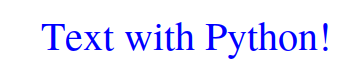
\includegraphics[scale=0.6]{../markdown/screen-markdown-7-en}
\end{center}
The code is:
\begin{lstlisting}
from tkinter import *
from tkinter.font import Font
# tkinter window
root = Tk()  
canvas = Canvas(root, width=800, height=600, background="white")
canvas.pack(fill="both", expand=True)
# Font
myfont = Font(family="Times", size=30)
# Some text
canvas.create_text(100,100, text="Text with Python!", 
anchor=SW, font=myfont, fill="blue")
# Launch the window
root.mainloop()
\end{lstlisting}


Some explanations:
\begin{itemize}
  \item \ci{root} and \ci{canvas} are the variables that define a graphic window (here of width $800$ and height $600$ pixels). This window is launched by the last command: \ci{root.mainloop()}.
  
  \item We remind you that for the graphic coordinates, the $y$-axis is directed downwards. To define a rectangle, simply specify the coordinates 
  $(x_1,y_1)$ and $(x_2,y_2)$ from two opposite vertices (see figure below). 
  
  \item The text is displayed by the command \ci{canvas.create_text()}. It is necessary to specify the $(x,y)$ coordinates of the point from which you want to display the text. 
  
  \item The \ci{text} option allows you to pass the string to display.
  
  \item The \ci{anchor} option allows you to specify the text anchor point, \ci{anchor=SW} means that the text box is anchored to the Southwest point (\emph{SW}) (see figure below).
  
  \item The \ci{fill} option allows you to specify the text color.
  
  \item The \ci{font} option allows you to define the font (i.e. the style and size of the characters). Here are some examples of fonts, it's up to you to test them:
  \begin{itemize}
    \item \ci{Font(family="Times", size=20)} 
    \item \ci{Font(family="Courier", size=16, weight="bold")} in \textbf{bold}
    \item \ci{Font(family="Helvetica", size=16, slant="italic")} in \emph{italic}
  \end{itemize}  
\end{itemize}

\myfigure{0.7}{
\tikzinput{screen-markdown-8-en}
}




%---------------------------------------------------
\subsection{Mouse click}

Here is a small program that displays a graphic window. Each time the user clicks (with the left mouse button) the program displays a small square (on the window) and displays \og{}Click at $x=\ldots$, $y=\ldots$\fg{} (on the console).

\begin{lstlisting}
from tkinter import *

# Window
root = Tk()
canvas = Canvas(root, width=800, height=600, background="white")
canvas.pack(side=LEFT, padx=5, pady=5)

# Catch mouse click
def action_mouse_click(event):
    canvas.focus_set()
    x = event.x
    y = event.y
    canvas.create_rectangle(x,y,x+10,y+10,fill="red")
    print("Click at x =",x,", y =",y)
    return

# Association click/action
canvas.bind("<Button-1>", action_mouse_click)

# Launch
root.mainloop()
\end{lstlisting}


Here are some explanations:
\begin{itemize}
  \item The creation of the window is usual. The program ends with the launch using the command  \ci{mainloop()}.
  
  \item The first key point is to associate a mouse click to an action, that's what the line does: 
\mycenterline{\ci{canvas.bind("<Button-1>", action_mouse_click)}}

Each time the left mouse button is clicked, \Python{} executes the \ci{action_mouse_click} function. (Note that there are no brackets for the call to the function.)

   \item Second key point: the \ci{action_mouse_click} function retrieves the click coordinates and then does two things here: it displays a small rectangle at the click location and prints the $(x,y)$ coordinates in the terminal window.
   
   \item The coordinates $x$ and $y$ are expressed in pixels; $(0,0)$ refers to the upper left corner of the window (the area delimited by \ci{canvas}).
\end{itemize}


%---------------------------------------------------
\subsection{Movement}

Here is a program that moves a small square and bounces it off the edges of the window.

\begin{center}
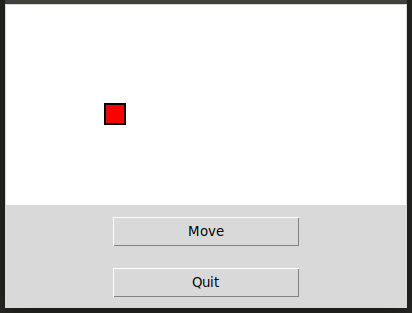
\includegraphics[scale=\myscale,scale=0.5]{../blocks/screen-blocks-lesson-move-en}
\end{center}

Here are the main points:
\begin{itemize}
  \item An object \ci{rect} is defined, it is a global variable, as well as its coordinates \ci{x0}, \ci{y0}.
  
  \item This object is (a little bit) moved by the function \ci{mymove()} which shifts the rectangle by \ci{(dx,dy)}.
    
  \item The key point is that this function will be executed again after a short period of time. The command: 
  \mycenterline{\ci{canvas.after(50,mymove)}}  
  requests a new execution of the function \ci{mymove()} after a short delay (here $50$ milliseconds).
  
  \item The repetition of small shifts simulates movement.
\end{itemize}

\begin{lstlisting}
from tkinter import *

the_width = 400
the_height = 200

root = Tk()     
canvas = Canvas(root,width=the_width,height=the_height,background="white")
canvas.pack(fill="both", expand=True)

# Coordinates and speed
x0, y0 = 100,100
dx = +5  # Horizontal speed
dy = +2  # Vertical speed

# The rectangle to move
rect = canvas.create_rectangle(x0,y0,x0+20,y0+20,width=2,fill="red")

# Main function
def mymove():
    global x0, y0, dx, dy

    x0 = x0 + dx  # New abscissa
    y0 = y0 + dy  # New ordinate

    canvas.coords(rect,x0,y0,x0+20,y0+20)  # Move

    if x0 < 0 or x0 > the_width:
        dx = -dx  # Change of horizontal direction
    if y0 < 0 or y0 > the_height:
        dy = -dy  # Change of vertical direction

    canvas.after(50,mymove)  # Call after 50 milliseconds
 
    return
    
# Function for the button
def action_move():
    mymove()
    return

# Buttons
button_move = Button(root,text="Move", width=20, command=action_move)
button_move.pack(pady=10)

button_quit = Button(root,text="Quit", width=20, command=root.quit)
button_quit.pack(side=BOTTOM, pady=10)

root.mainloop()
\end{lstlisting}


\end{document}
